\lab{Python}{Object Oriented Programming}{Object Oriented Programming}
\label{lab:OOP}
\objective{Teach how to use OOP in Python and illustrate the uses of OOP in programming graphical user interfaces}

\section*{Programming Paradigms}
There are many different styles of program organization.
A way of organizing a program is often called a ``paradigm."
These paradigms are designed to create better code by structuring or organizing the code in a more meaningful way.
Code without any structure is often referred to as ``spaghetti code.''
Spaghetti can be very easy to write, but very difficult to understand or modify.
It is good practice to structure your programs in such a way that they are easy to understand, extend, or reuse.
Making extensive use of procedures (or subfunctions) is a characteristic of \emph{procedural programming}.
The work of the program is done in the subfunctions with one main function supervising the calling of each subfunction.
\emph{Structured programming} emphasizes the use of programming structures to select or repeat the execution of blocks of code.
Another important, albeit specialized, paradigm is \li{object oriented programming} (or OOP).
The concept of object oriented programming is to model a problem as the interaction of a collection of objects.
There are many other paradigms such as declarative, event-driven, and array programming.

In this lab we will first learn how to create a class and then use Python and Qt4 (with bindings provided by PySide or PyQt) to create a web navigator.
It will be able to load and render webpages and will have basic navigation functionality such as back, forward, stop, and reload.
This project is designed to be used for demonstration purposes only and no effort is made to make this program secure.

\section*{Fundamental Concepts}
At its core, object oriented programming relies on the manipulation and coordination of objects.
An object represents a piece of code that tracks a state and provides methods for discovering or altering the state.
For example, think of a die.
We can create an object that would represent our die.
There would be a variable that keeps track of the current side facing up.
We would define a method, \li{roll()}, that would simulate rolling the die by randomly choosing an integer between 1 and 6.
Whenever \li{roll()} is called, it would update the variable tracking the current side facing up before returning.
We could have another method named \li{peek()} that would let us look at the current side facing up without changing it.
A code representation of our die would look something like
\begin{lstlisting}
class Die(object):
    def __init__(self):
        self.face = random.randint(1, 6)
    def roll(self):
        self.face = random.randint(1, 6)
        return self.peek()
    def peek(self):
        return self.face
\end{lstlisting}

There are a few concepts that define object oriented programming

\begin{itemize}

\item Abstraction - appropriate representation of states and data

\item Encapsulation - independent behavior

\item Inheritance - relations between objects

\end{itemize}

The general advantage of using these concepts is that it helps with organizing code.
``Abstraction" permits the presentation of only necessary details about an object to the user.
For example, when we ask someone if they own a computer, we can use abstraction to ask the question ``Do you own a computer?'' rather than asking about each and every combination of hardware that we could classify as a computer.
Inheritance helps us easily achieve this abstraction.
We could have an object called \li{Computer}.
Various brands would then subclass, or inherit, the properties of \li{Computer}.
We could continue by having each product line inherit from their respective brands, until we arrive at the product level.
Then each individual product would represent an instantiation of that product's class.
%Need graphic
Encapsulation means each function contains all of the data it needs to calculate a result.
Encapsulation is used to avoid the use of global data structures and makes managing data involved in computation more convenient.

Object oriented programming has gained popularity for many years.
Most modern programming languages support object oriented programming concepts.
Python is no exception.
In fact, everything in Python is an object.
We can create our own objects in Python by defining a \emph{class}.
A class is a blueprint that describes how to create an object.
\begin{lstlisting}
class Backpack(object):
    pass
\end{lstlisting}
We now have a class \li{Backpack} which contains nothing.
We can create \li{Backpack} objects by running something like \li{b = Backpack()}, but we can't really do anything with them.
The variable \li{b} is now an \emph{instance} of type \li{Backpack}.
Let's define an initial state for our object.
\begin{lstlisting}
class Backpack(object):
    def __init__(self):
        self.color = 'black'
\end{lstlisting}
Let's explain what's going on here.
The \li{self} is a reference to the current instance of the class.
All class methods take a reference to the current instance of the class as their first argument.
It is a very established convention to name this parameter \li{self}.
The \li{__init__} method is defined for all objects and is executed immediately after the object is created.
Its purpose is to set the initial state of the object.
In our backpack object, we set the color to black.
Thus all backpack objects will have the color black.
Let's have the user instantiate with a desired color
\begin{lstlisting}
class Backpack(object):
    def __init__(self, color='black'):
        self.color = color
        self.contents = []
\end{lstlisting}
We can instantiate a \li{Backpack} object of the color purple.
\begin{lstlisting}
b = Backpack(color='purple')
a = Backpack()
print b.color #prints `purple'
print a.color #prints `black'
\end{lstlisting}
The variable \li{self.color} is an instance variable.
It is defined for a particular instance of a backpack.
Finally, lets add some methods.
\begin{lstlisting}
class Backpack(object):
    def __init__(self, color='black'):
        self.color = color
        self.contents = []
        
    def put(self, item):
        self.contents.append(item)
        
    def take(self, item):
        return self.contents.pop(self.contents.index(item))
        
    def __repr__(self):
        return str(self.contents)
\end{lstlisting}
The \li{\_\_repr\_\_} method defines how to represent the class as a string and is one example of a magic method.
Magic methods are used for many purposes, some of the most useful ones include defining how to handel operators such as $ =, - , >, <$ and so on.
For more information on creating methods and magic methods read \url{http://www.rafekettler.com/magicmethods.html}.
This information may be helpful in solving Problem \ref{prob:complexNum}.

We now have a complete model of a backpack and can put in items and remove them as needed.

\begin{lstlisting}
b = Backpack(color='green')
print b.color #prints `green'
b.color = 'turqoise' # we can change an instance variable at any time
print b.color #prints `turqoise'
b.put(5)
b.put(3)
b.put(9)
b.put(1)
print b #prints `[5, 3, 9, 1]'
b.take(3)
print b #prints `[5, 9, 1]'
\end{lstlisting}


\begin{problem}
Create a \li{ComplexNumber} object that supports the basic operations of a complex number.
You must implement methods that will compare, add, subtract, multiply, divide, and conjugate complex numbers.
Also, implement a \li{norm()} method that will calculate the euclidean distance between two points on the complex plane.
\label{prob:complexNum}
\end{problem}

\section*{Building a Web Navigator}
Now that we know that basics of creating classes, we will use these to create a web navigator.
First, we need to import the libraries we will need for this project.
Qt, the framework we will leverage, is a cross-platform application framework.
It is very comprehensive and powerful and supports a number of platforms including Linux, OS X, Windows, etc.
At the time of writing, PyQt and PySide support Qt version 4.8.
\begin{lstlisting}
import sys
from PySide import QtCore, QtGui
from PySide import QtWebKit
\end{lstlisting}

\emph{Widgets} in Qt are objects that represent various elements of a GUI.
These widgets take care of drawing and refreshing the graphical display of the element as well as abstracting the behavior and defining ways to interact with the widget.
We are going to create our own widget, called \li{WebNavigator}, that will represent a simple web navigator.
We start by inheriting all the properties and methods of a generic widget.
\begin{lstlisting}
class WebNavigator(QtGui.QWidget):
    def __init__(self, home="about:blank"):
        super(WebNavigator, self).__init__()
        self.home = QtCore.QUrl(home)
\end{lstlisting}
The \li{super()} method refers to the superclass (the class we inherited from).
We use it to call the \li{\_\_init\_\_()} method of the parent class which in this case is \li{QtGui.QWidget}.
The Qt widgets that we will use to build our web navigator are: \li{QtWebkit}, \li{QtProgressBar}, \li{QtLineEdit}, and \li{QtPushButton}.
Let's begin by adding the core component, \li{QWebView}, to our widget.
This widget is able to load and render web content using WebKit.
WebKit is a popular layout rendering engine that is used in Safari and Google Chrome (up til version 27).
\begin{lstlisting}
class WebNavigator(QtGui.QWidget):
    def __init__(self, home="about:blank"):
        super(WebNavigator, self).__init__()
        self.home = QtCore.QUrl(home)
        self._initUI()
    def _initUI(self):
        self.wkctl = QtWebKit.QWebView(self)
        self.wkctl.setUrl(self.home)
        self.wkctl.urlChanged.connect(self.changedURL)
\end{lstlisting}
We need a reference pointing to our newly created \li{QWebView} widget so we can access it outside of \li{\_initUI()}.
We set the URL of our web view widget to be a predefined home page.  
The last line illustrates the power of object oriented design.
How to you handle user interaction with widgets?
How do you know if certain events have occurred?
Qt uses a system of \emph{signals} and \emph{slots}.
Signals are emitted by objects when a particular event occurs.
Slots receive signals perform some action based on the signal received.
In our code above, \li{urlChanged()} is a signal sent by \li{self.wbctl} to the method \li{self.changedURL} (the slot).
The slot can be any callable function in Python.
So we should define \li{changedURL()}.
\begin{lstlisting}
def changedURL(self, url):
    self.addr_bar.setText(url.toString())
\end{lstlisting}
Now whenever the URL of our web view changes, \li{changedURL()} is called and passed the new URL (as part of the signal).
Our function, which is a method of \li{WebNavigator}, accepts this new URL and changes the contents of the address bar.
At least, that is what we want it to do.
We need to add an address bar.
\begin{lstlisting}
def _initUI(self):
    self.wkctl = QtWebKit.QWebView(self)
    self.wkctl.setUrl(self.home)
    self.wkctl.urlChanged.connect(self.changedURL)
    
    self.addr_bar = QtGui.QLineEdit(self)
    self.addr_bar.setText(self.home.toString())
    self.addr_bar.returnPressed.connect(self.goURL)
def goURL(self):
    new_addr = QtCore.QUrl.fromUserInput(self.addr_bar.text())
    self.wkctl.load(new_addr)
\end{lstlisting}
Our address bar is a \li{QLineEdit} widget that will send a signal to \li{goURL()} whenever return is pressed inside the widget.
This event will trigger the web view to load the contents of the address bar parsed as a URL.
Let's finish creating and connecting the rest of the widgets we need.
\begin{lstlisting}
def _initUI(self):
    self.wkctl = QtWebKit.QWebView(self)
    self.wkctl.setUrl(self.home)
    self.wkctl.urlChanged.connect(self.changedURL)
    
    self.addr_bar = QtGui.QLineEdit(self)
    self.addr_bar.setText(self.home.toString())
    self.addr_bar.returnPressed.connect(self.goURL)
    
    prog_bar = QtGui.QProgressBar(self)
    self.wkctl.loadProgress.connect(prog_bar.setValue)
    
    back = QtGui.QPushButton("Back", self)
    back.clicked.connect(self.wkctl.back)
    
    forward = QtGui.QPushButton("Forward", self)
    forward.clicked.connect(self.wkctl.forward)
    
    self.stop_reload = QtGui.QPushButton("Reload", self)
    self.wkctl.loadStarted.connect(self.stop_action)
    self.wkctl.loadFinished.connect(self.reload_action)
    
    go_button = QtGui.QPushButton("Go!", self)
    go_button.clicked.connect(self.goURL)
    
    self.setGeometry(0, 0, 1024, 768)
    self.setWindowTitle("Simple WebKit Navigator")
    self.show()
def stop_action(self):
    self.stop_reload.setText("Stop")
    self.stop_reload.clicked.connect(self.wkctl.stop)
def reload_action(self):
    self.stop_reload.setText("Reload")
    self.stop_reload.clicked.connect(self.wkctl.reload)
\end{lstlisting}
We can see the result of our program in Figure \ref{fig:nolayout}.
Notice how the widgets are just stacked on top of each other.
Qt defines various layout widgets that allow us to control the placement of widgets. 
\begin{figure}[h]
\centering
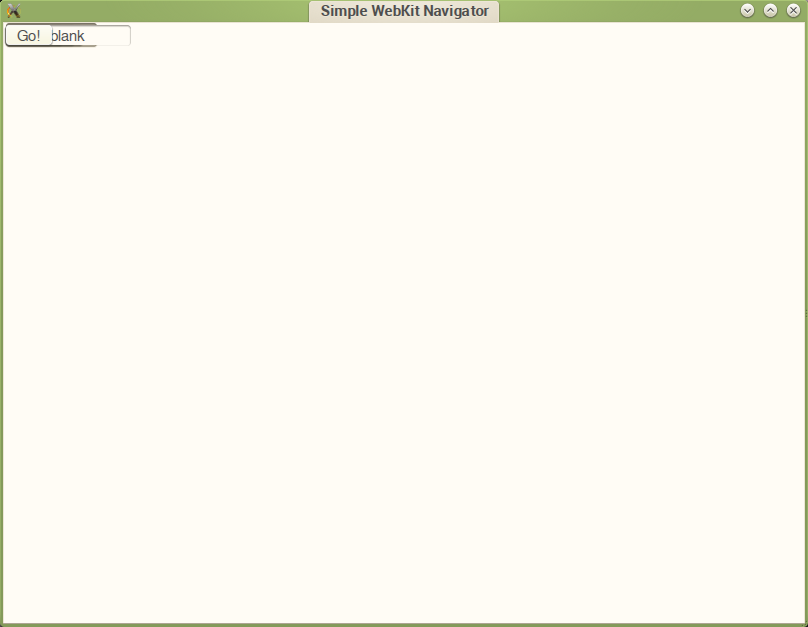
\includegraphics[scale=.5]{nolayout.png}
\caption{Application with no layout specified.}
\label{fig:nolayout}
\end{figure}
We are going to use two layouts in our web navigator widget: \li{QHBoxLayout} and \li{QVBoxLayout}.
There are also layouts for grids and forms.
In the \li{\_initUI()} method we need to append before \li{self.show()}
\begin{lstlisting}
navbar = QtGui.QHBoxLayout()
navbar.addWidget(back)
navbar.addWidget(forward)
navbar.addWidget(self.stop_reload)
navbar.addWidget(self.addr_bar)
navbar.addWidget(go_button)

vbox = QtGui.QVBoxLayout()
vbox.addLayout(navbar)
vbox.addWidget(self.wkctl)
vbox.addWidget(prob_bar)

self.setLayout(vbox)
\end{lstlisting}
Adding the layouts yields results in Figure \ref{fig:withlayout}.
\begin{figure}[h]
\centering
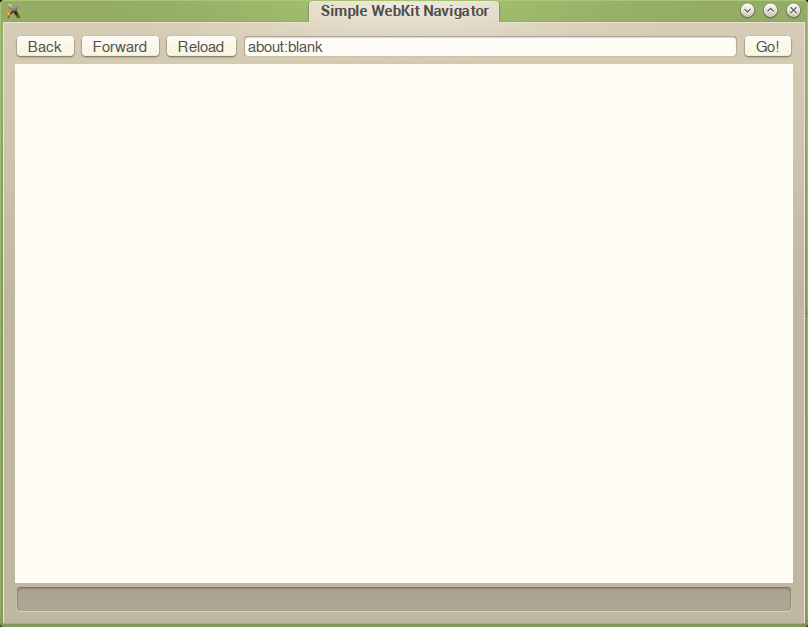
\includegraphics[scale=.5]{layout.png}
\caption{Application using a nested layout.
The controls in the navigation bar have their own layout which is nested into the first spot of the application-wide layout.}
\label{fig:withlayout}
\end{figure}

Structuring our program as a class allows us to very cleanly initialize a new application.
\begin{lstlisting}
def main():
    app = QtGui.QApplication(sys.argv)
    web = WebNavigator()
    sys.exit(app.exec_())
\end{lstlisting}
We first define a \li{QApplication} instance.
There can only a single \li{QApplication} object in existence at any time.
It initializes the context for all QWidget based applications.
It also manages the windows of the application and handles user input.
Next we instantiate our \li{WebNavigator} widget.
The last line starts the event handling loop and will exit Python when the application is terminated.
The completed program is listed below.
\lstinputlisting[style=fromfile]{webby.py}

\begin{problem}
Create a simple graphical user interface that will solve the quadratic formula given the necessary parameters.
Make the GUI look as below.
\begin{figure}[H]
\centering
\begin{subfigure}[b]{.49\textwidth}
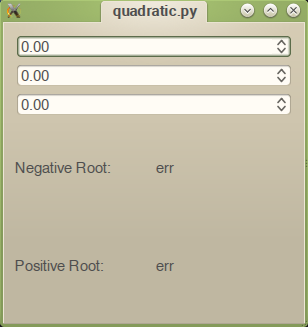
\includegraphics[width=\textwidth]{quadratic_view.png}
\end{subfigure}
\begin{subfigure}[b]{.49\textwidth}
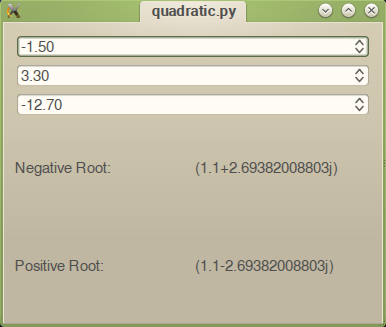
\includegraphics[width=\textwidth]{quadratic_view2.png}
\end{subfigure}
\end{figure}
The widgets that you will need are: \li{QDoubleSpinBox}, \li{QLabel}, \li{QGridLayout}, and \li{QVBoxLayout}.
You can view the documentation for these classes including all methods and signals at \url{http://qt-project.org/doc/qt-4.8/classes.html}
\end{problem}

\section*{Solutions}

The following is a guideline for your solutions.
\begin{lstlisting}
import sys
from Pyside import QtGui, QtCore, QtWebKit

class ComplexNumber(object):
	pass
	
class QuadraticCalculator(QtGui.QWidget):
	pass
\end{lstlisting}

